\section{Заключение}
	\begin{figure}
		\centering
		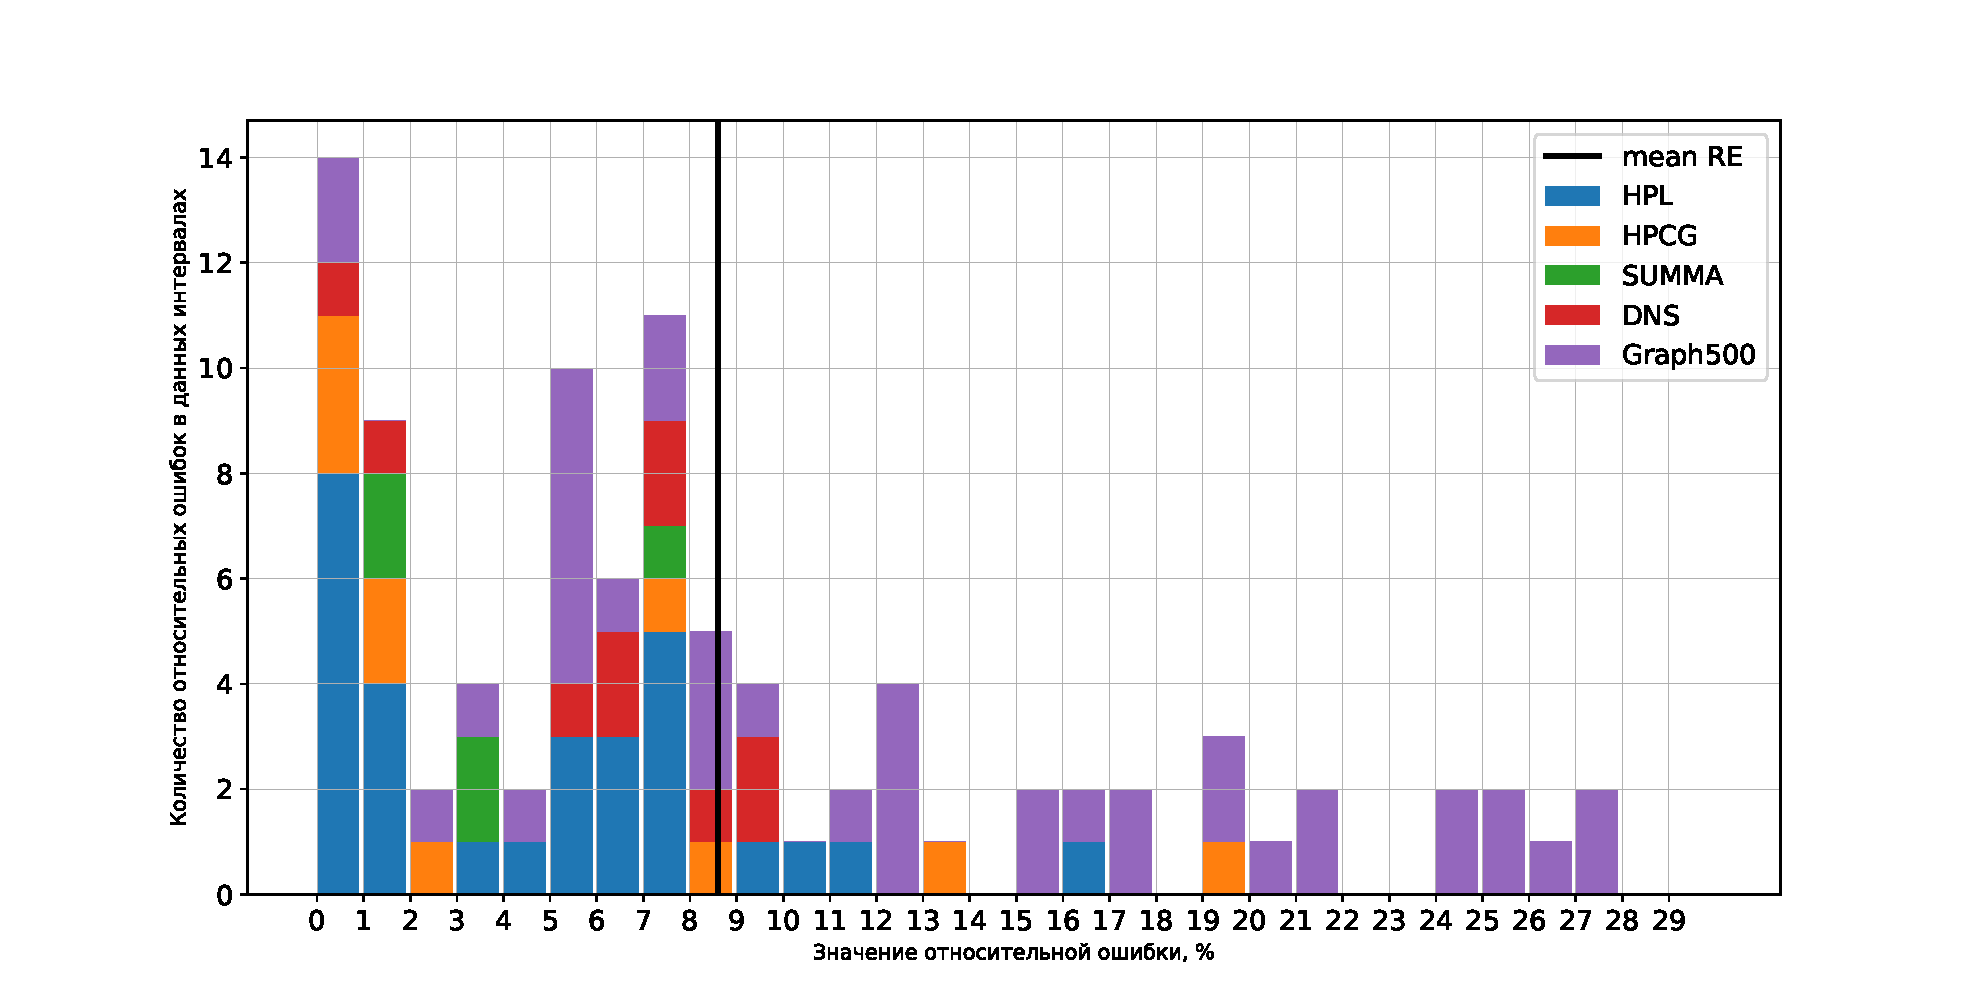
\includegraphics[width=\textwidth]{./images/RE_graph}
		\caption{Относительные ошибки предсказаний по всем рассматриваемым приложениям}
		\label{RESULT}
	\end{figure}
	В данной работе были получены следующие основные результаты:
	\begin{itemize}
		\item Разработан метод, предсказывающий слабую масштабируемость суперкомпьютерных приложений на основе экспериментальных данных.
		\item Выполнена проверка применимости метода на различных приложениях, с помощью запусков приложений HPL, HPCG, матричных алгоритмов умножения SUMMA и DNS, Graph500 на суперкомпьютере "<Ломоносов-2">.
	\end{itemize}

	На основании предложенного метода удалось построить предсказания слабой масштабируемости для всех рассматриваемых приложений так, что максимальная относительная ошибка среди всех приложений и конфигураций не превышает 28\%, однако подобный значения являются единичными случаями. Средние значения относительных ошибок для различных приложений равны HPL - 4,9\%, HPCG - 5,6\%, SUMMA - 3,6\%, DNS - 6,4\%, Graph500 - 13,2\%. Так как почти четверть всех предсказаний значений динамических характеристик приходится на Graph500, а именно на этом приложении сильнее всего отразились трудности заданием конфигураций запусков, поэтому значения относительных именно на этом приложении во многом являются определяющими, при расчёте среднего значения ошибок по всем приложениям, которое составляет 8,6\%. Гистограмма с различными значениями относительных ошибок представлена на рисунке \eqref{RESULT}. Таким образом, предложенный метод предсказания даёт относительные ошибки, сравнимые с ошибками предсказания у существующих подходов при сопоставимых размерах конфигураций предсказываемых запусков. Но отличается от них простотой построения, отсутствием необходимости собирать большой набор тестовых данных. Помимо этого, он удовлетворяет поставленным условиям универсальности.
	
\clearpage
%\newpage